% Created by tikzDevice version 0.12.3 on 2019-12-11 20:53:26
% !TEX encoding = UTF-8 Unicode
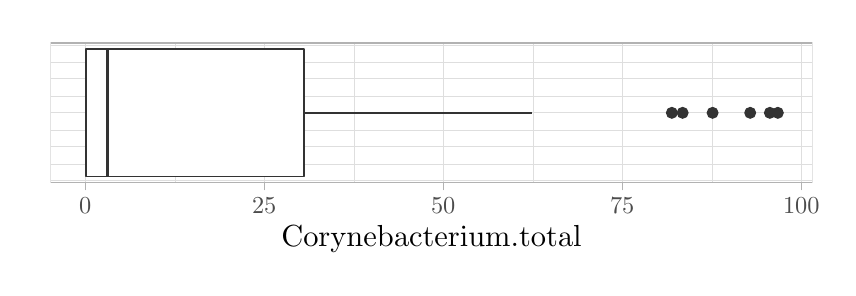
\begin{tikzpicture}[x=1pt,y=1pt]
\definecolor{fillColor}{RGB}{255,255,255}
\path[use as bounding box,fill=fillColor,fill opacity=0.00] (0,0) rectangle (289.08, 86.72);
\begin{scope}
\path[clip] (  0.00,  0.00) rectangle (289.08, 86.72);
\definecolor{drawColor}{RGB}{255,255,255}
\definecolor{fillColor}{RGB}{255,255,255}

\path[draw=drawColor,line width= 0.6pt,line join=round,line cap=round,fill=fillColor] (  0.00,  0.00) rectangle (289.08, 86.72);
\end{scope}
\begin{scope}
\path[clip] (  8.25, 30.69) rectangle (283.58, 81.22);
\definecolor{fillColor}{RGB}{255,255,255}

\path[fill=fillColor] (  8.25, 30.69) rectangle (283.58, 81.22);
\definecolor{drawColor}{gray}{0.87}

\path[draw=drawColor,line width= 0.1pt,line join=round] (  8.25, 37.58) --
	(283.58, 37.58);

\path[draw=drawColor,line width= 0.1pt,line join=round] (  8.25, 49.83) --
	(283.58, 49.83);

\path[draw=drawColor,line width= 0.1pt,line join=round] (  8.25, 62.08) --
	(283.58, 62.08);

\path[draw=drawColor,line width= 0.1pt,line join=round] (  8.25, 74.33) --
	(283.58, 74.33);

\path[draw=drawColor,line width= 0.1pt,line join=round] ( 53.11, 30.69) --
	( 53.11, 81.22);

\path[draw=drawColor,line width= 0.1pt,line join=round] (117.81, 30.69) --
	(117.81, 81.22);

\path[draw=drawColor,line width= 0.1pt,line join=round] (182.50, 30.69) --
	(182.50, 81.22);

\path[draw=drawColor,line width= 0.1pt,line join=round] (247.19, 30.69) --
	(247.19, 81.22);

\path[draw=drawColor,line width= 0.3pt,line join=round] (  8.25, 31.45) --
	(283.58, 31.45);

\path[draw=drawColor,line width= 0.3pt,line join=round] (  8.25, 43.70) --
	(283.58, 43.70);

\path[draw=drawColor,line width= 0.3pt,line join=round] (  8.25, 55.95) --
	(283.58, 55.95);

\path[draw=drawColor,line width= 0.3pt,line join=round] (  8.25, 68.21) --
	(283.58, 68.21);

\path[draw=drawColor,line width= 0.3pt,line join=round] (  8.25, 80.46) --
	(283.58, 80.46);

\path[draw=drawColor,line width= 0.3pt,line join=round] ( 20.77, 30.69) --
	( 20.77, 81.22);

\path[draw=drawColor,line width= 0.3pt,line join=round] ( 85.46, 30.69) --
	( 85.46, 81.22);

\path[draw=drawColor,line width= 0.3pt,line join=round] (150.15, 30.69) --
	(150.15, 81.22);

\path[draw=drawColor,line width= 0.3pt,line join=round] (214.85, 30.69) --
	(214.85, 81.22);

\path[draw=drawColor,line width= 0.3pt,line join=round] (279.54, 30.69) --
	(279.54, 81.22);
\definecolor{drawColor}{gray}{0.20}
\definecolor{fillColor}{gray}{0.20}

\path[draw=drawColor,line width= 0.4pt,line join=round,line cap=round,fill=fillColor] (268.19, 55.95) circle (  1.96);

\path[draw=drawColor,line width= 0.4pt,line join=round,line cap=round,fill=fillColor] (232.77, 55.95) circle (  1.96);

\path[draw=drawColor,line width= 0.4pt,line join=round,line cap=round,fill=fillColor] (261.08, 55.95) circle (  1.96);

\path[draw=drawColor,line width= 0.4pt,line join=round,line cap=round,fill=fillColor] (247.49, 55.95) circle (  1.96);

\path[draw=drawColor,line width= 0.4pt,line join=round,line cap=round,fill=fillColor] (271.06, 55.95) circle (  1.96);

\path[draw=drawColor,line width= 0.4pt,line join=round,line cap=round,fill=fillColor] (236.67, 55.95) circle (  1.96);

\path[draw=drawColor,line width= 0.6pt,line join=round] ( 99.89, 55.95) -- (182.12, 55.95);

\path[draw=drawColor,line width= 0.6pt,line join=round] ( 21.13, 55.95) -- ( 20.77, 55.95);
\definecolor{fillColor}{RGB}{255,255,255}

\path[draw=drawColor,line width= 0.6pt,line join=round,line cap=round,fill=fillColor] ( 99.89, 32.98) --
	( 21.13, 32.98) --
	( 21.13, 78.93) --
	( 99.89, 78.93) --
	( 99.89, 32.98) --
	cycle;

\path[draw=drawColor,line width= 1.1pt,line join=round] ( 29.00, 32.98) -- ( 29.00, 78.93);
\definecolor{drawColor}{gray}{0.70}

\path[draw=drawColor,line width= 0.6pt,line join=round,line cap=round] (  8.25, 30.69) rectangle (283.58, 81.22);
\end{scope}
\begin{scope}
\path[clip] (  0.00,  0.00) rectangle (289.08, 86.72);
\definecolor{drawColor}{gray}{0.70}

\path[draw=drawColor,line width= 0.3pt,line join=round] ( 20.77, 27.94) --
	( 20.77, 30.69);

\path[draw=drawColor,line width= 0.3pt,line join=round] ( 85.46, 27.94) --
	( 85.46, 30.69);

\path[draw=drawColor,line width= 0.3pt,line join=round] (150.15, 27.94) --
	(150.15, 30.69);

\path[draw=drawColor,line width= 0.3pt,line join=round] (214.85, 27.94) --
	(214.85, 30.69);

\path[draw=drawColor,line width= 0.3pt,line join=round] (279.54, 27.94) --
	(279.54, 30.69);
\end{scope}
\begin{scope}
\path[clip] (  0.00,  0.00) rectangle (289.08, 86.72);
\definecolor{drawColor}{gray}{0.30}

\node[text=drawColor,anchor=base,inner sep=0pt, outer sep=0pt, scale=  0.88] at ( 20.77, 19.68) {0};

\node[text=drawColor,anchor=base,inner sep=0pt, outer sep=0pt, scale=  0.88] at ( 85.46, 19.68) {25};

\node[text=drawColor,anchor=base,inner sep=0pt, outer sep=0pt, scale=  0.88] at (150.15, 19.68) {50};

\node[text=drawColor,anchor=base,inner sep=0pt, outer sep=0pt, scale=  0.88] at (214.85, 19.68) {75};

\node[text=drawColor,anchor=base,inner sep=0pt, outer sep=0pt, scale=  0.88] at (279.54, 19.68) {100};
\end{scope}
\begin{scope}
\path[clip] (  0.00,  0.00) rectangle (289.08, 86.72);
\definecolor{drawColor}{RGB}{0,0,0}

\node[text=drawColor,anchor=base,inner sep=0pt, outer sep=0pt, scale=  1.10] at (145.91,  7.64) {Corynebacterium.total};
\end{scope}
\end{tikzpicture}
